\section{{{\fontsize{17}{21}\selectfont \textbf{Methodology and Working}}}}
\setlength{\columnsep}{1.5cm}
\vspace{0.5cm}
\begin{figure}[h]
  \centering
  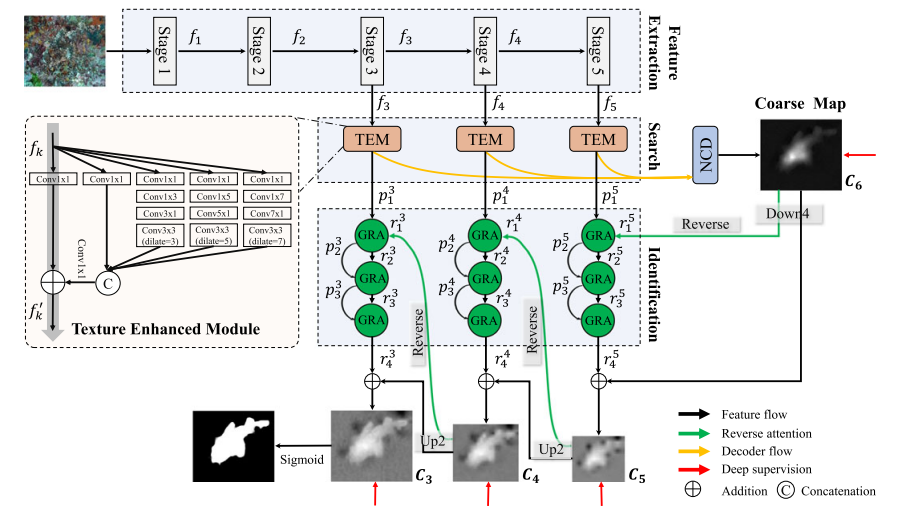
\includegraphics[width=0.9\textwidth,height=10cm]{sections/LBP/sinet.png}
  \caption{Pipeline of our SINet framework}
  \label{fig:figure_label}
\end{figure}

\begin{multicols}{2}
This section provides a detailed overview of the techniques and algorithms utilized in our project. By discussing the different methods applied, we aim to provide a better understanding of the approach taken to achieve the project's objectives.
\vspace{0.5cm}
\subsection{{{\fontsize{14}{19}\selectfont \textbf{COD Framework}}}}
\vspace{0.5cm}
\subsubsection{{{\fontsize{13}{17}\selectfont \textbf{Network Overview}}}}
The proposed framework for object detection is SINet\cite{inproceedings}(Search Identification Network). Now taking an overview of the network.\\
Several methods have shown that satisfactory performance is dependent on the re-optimization strategy (i.e., coarse-to-fine), which is regarded as the composition of multiple sub-steps. This also suggests that decoupling
the complicated targets can break the performance bottleneck. Our SINet model consists of the first two stages of hunting, i.e., search and identification. Specifically, the former phase is responsible for searching for a concealed object, while the latter one is then used to precisely detect
the concealed object in a cascaded manner.\\
The architecture consists of three main modules :\\ 
a) the texture Enhanced Module (TEM) which is used to capture fine-grained textures with the enlarged context cues.
b) The Neighbor connection Decoder (NCD), which is able to provide the location information
c) The Cascaded Group-Reversal Attention (GRA) blocks, which work collaboratively to refine the coarse prediction from the deeper layer.
\vspace{0.5cm}
\subsubsection{{{\fontsize{13}{17}\selectfont \textbf{Feature Extraction}}}}
For an input image \(\textbf{I}\epsilon  R^{W*H*3} \), a set of features \(f_k, k\epsilon \{1, 2, 3, 4, 5\} \) is extracted from Res2Net-50 (removing the top three layers, i.e., 'average pool', '1000d fc', and 'softmax'). Thus, the resolution of each feature \(f_k\) is \(H/2^k * W/2^k, k \epsilon \{1, 2, 3, 4, 5\}, \) covering diversified feature pyramids from high-resolution, weakly semantic to low-resolution, strongly semantic.
\vspace{0.5cm}
\subsubsection{{{\fontsize{13}{17}\selectfont \textbf{Texture Enhanced Module (TEM)}}}}\cite{tem}
TEM is used to incorporate more discriminative feature representations during the searching stage (usually in a small/local space).\\
Each TEM component includes four parallel residual branches \(\{b_i, i = 1, 2, 3, 4\}\) with different dilation rates \(d\epsilon \{1, 3, 5, 7\}\) and a shortcut
branch. In each branch \(b_i\), the first convolutional layer utilizes a 1*1 convolution operation (Conv1*1) to reduce the channel size to 32. This is followed by two other layers: a (2i-1)*(2i-1) convolutional layer and a 3*3 convolutional layer with a specific dilation rate (2i-1) when \(i > 1\). Then, the first four branches \(b_i, i = \{1, 2, 3, 4\}\) are concatenated and the channel size is reduced to \textit{C} via a 3*3 convolution operation. We set \textit{C} = 32 in the default implementation of our network for time-cost trade-off. Finally, the identity shortcut branch is added in, then the whole module is fed to a ReLU function to obtain the output feature \(f'_k\). TEM add one more branch with a larger dilation rate to enlarge the receptive field and further replace the standard convolution with two asymmetric convolutional layers.
\vspace{0.5cm}
\subsubsection{{{\fontsize{13}{17}\selectfont \textbf{Neighbor Connection Decoder (NCD)}}}}\cite{book}
As low-level features consume more computational resources due to their larger spatial resolutions, but contribute less to performance we decide to aggregate only the top-three highest-level features \((i.e., f_k\epsilon R^{W/2^k*H/2^k*C}, k = 3, 4, 5)\) to obtain a more efficient learning capability, rather than taking all the feature pyramids into consideration. To be specific, after obtaining the candidate features from the three previous TEMs, in the search phase, we need to locate the concealed object.\\
However, there are still two key issues when aggregating multiple feature pyramids; namely, how to maintain semantic consistency within a layer and how to bridge the context across layers. Here, we propose to address these with the neighbor connection decoder (NCD). More specifically, we modify the partial decoder component (PDC) with a neighbor connection function and get three refined features \(f^{nc}_k=F_{NC}(f'_k; \textbf{W}^u_{NC}, k\epsilon \{3,4,5\}\) and \(u \epsilon \{1,2,3\})\). To ensure shape matching between candidate features, we utilize an upsampling (e.g., 2 times) operation before element-wise multiplication. Then, we feed\(f^{nc}_k, k\epsilon \{3,4,5\}\) into the neighbor
connection decoder (NCD) and generate the coarse location.
\vspace{0.5cm}
\subsubsection{{{\fontsize{13}{17}\selectfont \textbf{Group-Reversal Attention (GRA)}}}}\cite{attention}
Here, we introduce the residual learning process, termed the GRA block, with the assistance of both the reverse guidance and group guidance operation. We combine multiple GRA blocks to progressively refine the coarse prediction via different feature pyramids. Overall, each GRA block has three residual learning processes:\\
\textit{1)} We combine candidate features \(p^k_i\) and \(r^k_l\) via the group guidance operation and then use the residual stage to produce the refined features \(p^kk_{i+1}\). We only reverse the guidance prior in the first GRA block (i.e., when i = 1) in the default implementation. \\
\textit{2)} Then, we get a single channel residual guidance which is parameterized by learnable weights \(W^w_{GRA}\).\\
\textbf{3)} Finally, we only output the refined guidance, which serves as the residual prediction.
\vspace{0.5cm}
\subsubsection{{{\fontsize{13}{17}\selectfont \textbf{Learning Strategy}}}}
Our loss function is defined as \(L = L^W_{IoU} + L^W_{BCE}\), where \(L^W_{IoU}\) and \(L^W_{BCE}\)\cite{heera2019binary} represent the weighted intersection-over-union (IoU) loss and binary cross entropy (BCE) loss for the global restriction and local (pixel-level) restriction. Different from the standard IoU loss, the weighted IoU loss increases the weights of hard pixels to highlight their importance. In addition, compared with the standard BCE loss, \(L^W_{BCE}\) pays more attention to hard pixels rather than assigning all pixels equal weights. Here, we adopt deep supervision for the three side-outputs \((i.e., C_3, C_4, and C_5)\) and the global map \(C_6\). Each map is up-sampled (e.g., \(C^{up}_3\)) to the same size as the ground-truth map G. Thus, the total loss for the proposed SINet can be formulated as:\\
 \({L}_{total} = (\textit{L}(\textit{C}^{up}_6 , \textit{G}) + \sum^{i=5}_{i=3}\textit{L}(\textit{C}^{up}_i , \textit{G})\).
 
\vspace{0.5cm}
\subsection{{{\fontsize{14}{19}\selectfont \textbf{Using Drone Data}}}}
We are given images captured from drone where we have images of 5 different spectrum\cite{fusion} taken by different drones of the same environment. As there will be some difference in the orientation of drones, the 5 images obtained are also having some difference in their orientation. Our model is based on 3-channelled input so we aim to convert the 5-channel image of our drone data into 3-channelled image.For our purpose we first need to align our 5 images so that their is no noise when we combine the images. For that we use Image Registration Technique. After aligning the images we need to convert the 5-channelled aligned images to 3-channelled image. Our approach here is using PCA for it as PCA is unsupervised feature extraction technique which is simple to implement and give effective and efficient results. Hence, we use PCA to convert 5-featured data to 3-featured data. 

\vspace{0.5cm}
\subsubsection{{{\fontsize{13}{17}\selectfont \textbf{Image Registration}}}}\cite{image_reg}
Image registration is a technique used to align two or more images of the same scene taken from different viewpoints or at different times. The goal is to find a transformation that maps the pixels of one image to the corresponding pixels of the other image(s). This technique has numerous applications in computer vision, medical imaging, remote sensing, and many other fields.\\
There are several approaches to image registration, including feature-based methods, intensity-based methods, and hybrid methods.\\
Feature-based methods rely on identifying and matching distinctive features such as corners, edges, or blobs in the images. The transformation is then computed based on the matched features. This approach is robust to changes in lighting, contrast, and occlusion, but may fail when there are not enough distinctive features in the images.\\
Intensity-based methods use the intensity values of the images to compute the transformation. These methods optimize a similarity metric that measures the similarity between the images, such as mutual information or correlation. This approach is more general than feature-based methods but may be sensitive to changes in lighting and contrast.\\
Hybrid methods combine the advantages of feature-based and intensity-based methods. They first identify a set of features in the images, and then use the intensity values around the features to compute the transformation. This approach is more robust than either of the other methods alone.\\
In general, image registration is a challenging problem, especially when the images are noisy, contain artifacts, or have significant differences in scale, rotation, or perspective. However, with the appropriate techniques and algorithms, image registration can be a powerful tool for many applications.

\vspace{0.5cm}
\subsubsection{{{\fontsize{13}{17}\selectfont \textbf{Principle Component Analysis(PCA)}}}}
Principal Component Analysis (PCA) is a statistical technique used to reduce the dimensionality of a dataset by identifying the most significant features, known as principal components, that capture the majority of the variation in the data. This technique is commonly used in data preprocessing and feature extraction in machine learning, computer vision, and other fields.\\
The basic idea of PCA is to transform a high-dimensional dataset into a lower-dimensional space by projecting the data onto a new set of orthogonal axes that capture the maximum amount of variation in the data. The first principal component is the axis that captures the most variance in the data, and each subsequent principal component captures the remaining variance in decreasing order.\\
To compute the principal components, PCA finds the eigenvectors and eigenvalues of the covariance matrix of the data. The eigenvectors represent the directions of maximum variance in the data, while the eigenvalues represent the amount of variance captured by each eigenvector.\\
PCA can be used for various purposes, including data visualization, data compression, and feature extraction. In data visualization, PCA can be used to reduce the dimensionality of a high-dimensional dataset to two or three dimensions, allowing the data to be visualized in a scatter plot. In data compression, PCA can be used to reduce the size of the dataset while retaining most of the information. In feature extraction, PCA can be used to identify the most important features in the data and reduce the dimensionality of the feature space.\\
However, it is important to note that PCA assumes that the data is linearly related and that the principal components are uncorrelated. Therefore, it may not be suitable for all types of data, and other techniques such as nonlinear dimensionality reduction may be more appropriate in certain cases.
\end{multicols}

\vspace{0.5cm}
{\color{gray}\hrule}
\vspace{0.5cm}